%!TEX root = ../report.tex
\section{Preconditioning}

The iterative solver is $\textrm{CGSTAB}$ with $ILU$ as a preconditioner. The preconditioner has a single parameter $\epsilon$ which determines the drop tolerance in the incomplete decomposition. A value of $\epsilon = 0$ reduces to a full LU decomposition, which requires too much work and memory, and would make an iterative method superfluous. On the other hand, if $\epsilon = 1$ the preconditioner simply reduces to a diagonal matrix, which is cheap to apply, but maybe not as effective. Typically the optimal value for $\epsilon$ must be found experimentally. In our case it turns out $\epsilon \approx 10^{-6}$ is an optimal value in terms of CPU time spent on a single continuation step in $Re$ at $Re \approx 16$ and $\eta = 1$ (given the initial direction). See Figure~\ref{fig:optimal_epsilon} for reference.

\begin{figure}[h]
    \centerline{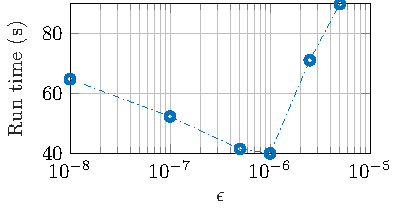
\includegraphics[width=\textwidth]{images/droptol_epsilon.pdf}}
    \caption{Finding the optimal drop tolerance paramter $\epsilon$ experimentally.}
    \label{fig:optimal_epsilon}
\end{figure}